\documentclass[conference]{IEEEtran}
\IEEEoverridecommandlockouts

\usepackage{cite}
\usepackage{amsmath,amssymb,amsfonts}
\usepackage{graphicx}
\usepackage{booktabs}
\usepackage{textcomp}
\usepackage{xcolor}
\usepackage[hidelinks]{hyperref}

\graphicspath{{figuras/}}

\begin{document}

\title{Cross-Site Transfer Learning versus Local Models for Short-Term Photovoltaic
Forecasting under Data Scarcity: A Leave-One-Plant-Out Benchmark on 94 Chilean Plants}

\author{\IEEEauthorblockN{C\'esar David Aular Mu\~noz}
\IEEEauthorblockA{School of Computer Engineering\\
Universidad Cat\'olica del Maule\\
Talca, Chile\\
Email: cesaraular02@gmail.com}}

\maketitle

\begin{abstract}
Newly commissioned photovoltaic (PV) plants lack the local generation history that
conventional forecasting models require, a \emph{Cold-Start} problem that translates into
operational and financial risk for grid operators and small distributed generators. We
investigate whether a single \emph{Cross-Site} deep-learning model, pretrained on many
consolidated plants, can forecast a brand-new plant it has never observed, and how it
compares against strictly local baselines. We benchmark eight configurations---global
Temporal Fusion Transformer (TFT), Informer, N-HiTS, LSTM and a global XGBoost against
strictly local XGBoost, LSTM and N-HiTS---under a Leave-One-Plant-Out (LOPO) protocol that
hides the target plant during training and seeds inference with a purely synthetic context
derived from a regional efficiency prior computed only on the training plants. Evaluation
spans 24-hour and autoregressive 7-day horizons over 94 Chilean plants (2014--2024), with
point (RMSE, sMAPE, rRMSE) and probabilistic (90\,\% interval coverage, pinball loss)
metrics, stratified by season. The results deliver a nuanced verdict. In absolute accuracy
the hypothesis is rejected: a mature local XGBoost (62\,\% median rRMSE, weekly roll-out)
beats the best global model (global XGBoost, 95\,\%). Yet at matched deep architecture,
global transfer is competitive---global LSTM (118\,\%) outperforms local LSTM
(147\,\%) despite never seeing the target. Winter is systematically the hardest season, and
the deep networks' probabilistic intervals are markedly miscalibrated under zero-shot
transfer. The Cross-Site approach is thus confirmed as operationally viable precisely where
the local paradigm cannot exist---the first hours after grid connection.
\end{abstract}

\begin{IEEEkeywords}
photovoltaic forecasting, transfer learning, cold-start, deep learning, Temporal Fusion
Transformer, probabilistic forecasting, leave-one-plant-out.
\end{IEEEkeywords}

\section{Introduction}
The accelerated deployment of solar photovoltaic (PV) generation confronts grid operators
with a recurrent operational barrier: a plant that has just been connected to the network
has no operating history from which to learn its production dynamics. Classical PV
forecasting pipelines train a dedicated model per plant on months or years of local
data~\cite{Antonanzas2016}; applied to a freshly commissioned facility they degrade sharply
or cannot be trained at all. This is the \emph{Cold-Start} problem, borrowed from
recommender systems~\cite{Schein2002}: reliable inference is required exactly when
site-specific evidence is absent. The resulting uncertainty inflates balancing costs and
financial exposure for system operators and, acutely, for the small distributed generators
that dominate the recent capacity additions.

A promising escape is to abandon the one-model-per-plant assumption. Instead of learning in
isolation, a single \emph{global} model can be trained across many plants simultaneously,
absorbing shared atmospheric-to-power patterns and transferring them to unseen
sites~\cite{MonteroManso2021,PanYang2010}. Modern attention-based sequence models---the
Temporal Fusion Transformer (TFT)~\cite{Lim2021}, Informer~\cite{Zhou2021}---and efficient
hierarchical alternatives such as N-HiTS~\cite{Challu2023} make this \emph{Cross-Site}
strategy technically feasible on multivariate, exogenous-rich PV data. The open question,
and the one this work addresses, is empirical and adversarial: \emph{under a strictly
zero-shot protocol, does a global Cross-Site model actually beat mature local baselines, or
does the transfer premium evaporate once the comparison is made fair?}

Much of the literature reports favourable global-transfer results but rarely combines three
demanding conditions at once: (i) a target-plant-blind evaluation with no local fine-tuning,
(ii) a direct contrast against mature local baselines under an identical protocol, and (iii)
a probabilistic characterization of the forecasts. We close this gap. Our contributions are:

\begin{itemize}
\item A reproducible LOPO benchmark of \textbf{eight configurations} (five global, three
strictly local) over \textbf{94 Chilean PV plants}, with formally verified zero-shot
integrity (no feature is a function of the target's own generation).
\item A \textbf{synthetic Cold-Start seeding} mechanism that initializes the inference
context from a regional efficiency prior computed exclusively on training plants, enabling
inference with zero target history without leakage.
\item A \textbf{point-and-probabilistic} evaluation stratified by season and by evaluation
window, exposing (a) the rejection of the global-superiority hypothesis in absolute terms,
(b) its nuance at matched architecture, (c) winter as the hardest regime, and (d) a
systematic miscalibration of the deep networks' intervals under transfer.
\end{itemize}

\section{Related Work}
\textbf{PV forecasting.} Deep networks consistently surpass classical statistical methods
for short-term PV power~\cite{Mellit2021,Kumari2021}, and on real solar datasets
attention-based models improve over classical machine learning at the cost of higher data
and compute demand~\cite{Arslan2025}. The TFT has been applied to day-ahead PV forecasting
with quantile outputs and interpretable covariate fusion~\cite{LopezSantos2022}. A recurrent
limitation across these works is the assumption of sufficient local history for training.

\textbf{Global vs.\ local forecasting.} Montero-Manso and Hyndman~\cite{MonteroManso2021}
formalize why a single global model fit across related series can generalize at least as
well as many local models, given enough cross-series signal. For intermittent series,
however, the balance between local and global models is not settled~\cite{Damato2026}, and
simple baselines often rival transformers on standard benchmarks~\cite{Zeng2023}---a caution
we find echoed in our PV results.

\textbf{Transfer learning for PV.} Bak et al.~\cite{Bak2025} pretrain on large multi-plant
corpora and fine-tune on the first records of a new site, attenuating error during the first
weeks of operation---but still requiring a local fine-tuning phase. Foundation-model
approaches push toward pure zero-shot irradiance transfer~\cite{Mishra2025}. Our study
differs by enforcing a strict zero-shot regime \emph{and} contrasting it, on the same
footing, against mature local baselines---a comparison typically absent from the transfer
literature.

\textbf{Probabilistic forecasting.} Quantile and distributional outputs are standard for
decision-relevant energy forecasting~\cite{Salinas2020,Benidis2022}. We adopt 90\,\%
prediction intervals and evaluate coverage and pinball loss, but crucially examine whether
calibration itself survives the zero-shot transfer.

\section{Methodology}

\subsection{Dataset and Medallion ETL}
The corpus comprises hourly generation from 94 PV plants of the Chilean National Electric
System (2014--2024), dynamic exogenous meteorology (global horizontal irradiance,
temperature, humidity) and static geographic attributes (macro-zone, installed capacity). A
Medallion pipeline (landing\,$\rightarrow$\,bronze\,$\rightarrow$\,silver\,$\rightarrow$\,gold)
parses raw meteorological CSVs, standardizes to a canonical
$(\mathit{unique\_id},\,\mathit{ds},\,y)$ schema, groups plants by macro-zone, engineers
cyclic calendar features and imputes \emph{only} exogenous variables (with an
\texttt{is\_imputed} dummy). Generation $y$ is never imputed: missing hours remain missing,
and metrics score real observations only.

\subsection{LOPO Protocol and Zero-Shot Integrity}
Evaluation follows a Leave-One-Plant-Out design. For each target plant, the global models
are trained on the full 2014--2024 history of the remaining $N{-}1$ plants; the target is
\emph{completely invisible} during training. Zero-shot integrity is a hard constraint: no
predictor may be a function of the target's own $y$. This is enforced by automated tests and
was decisive---an early efficiency prior computed per-row from the target
($\mathrm{corr}=1.0$ with $y$) produced a fake $\sim$0.8\,\% rRMSE that collapsed to the
honest $\sim$56\,\% once removed.

\subsection{Synthetic Cold-Start Context}
Deep models require a context window to initialize inference, which a new plant cannot
provide. We seed it synthetically:
\begin{equation}
\hat{y}_{\text{seed}}(t) = \mathrm{capacity}\cdot PR_{\text{regional}}\cdot s(t),
\end{equation}
where $s(t)$ is a deterministic solar profile and $PR_{\text{regional}}$ is a performance
ratio aggregated by macro-zone and season \emph{over the training plants only}. Only known or
forecastable exogenous weather and static geography use the target's real values; the
generation context is entirely synthetic (Fig.~\ref{fig:method}).

\subsection{Models and Probabilistic Output}
We evaluate five global configurations---TFT~\cite{Lim2021}, Informer~\cite{Zhou2021},
N-HiTS~\cite{Challu2023}, LSTM~\cite{Hochreiter1997} and a global gradient-boosted
XGBoost~\cite{Chen2016}---and three strictly local baselines (XGBoost, LSTM, N-HiTS) trained
only on the target's own history with all evaluation windows excluded. Deep models are
trained with NeuralForecast in \texttt{fp32} on a 6\,GB GPU; hyperparameters are tuned once
per model and reused across folds. Every model emits P5/P50/P95 quantiles (90\,\% intervals),
and predictions are physically constrained ($\hat{y}\!\geq\!0$; forced to zero at night).

\subsection{Evaluation Windows and Metrics}
\label{sec:windows}
Two horizons are scored: \emph{day1} (24\,h direct) and \emph{rollout7d} (7 autoregressive
days feeding back the predicted median). Because early series often contain a
\emph{commissioning ramp} of null generation, we report a window sensitivity analysis
(Fig.~\ref{fig:method}): \emph{Raw} (from the first recorded hour, ramp included),
\emph{Operational} (from first sustained production) and four \emph{Seasonal} windows
starting in each season, drawn from the plant's own later history. Point metrics are RMSE,
sMAPE and rRMSE (normalized by the window's mean hourly generation, which includes null night
hours and therefore inflates the index---its value is the \emph{relative} comparison across
architectures on identical windows). Probabilistic quality uses 90\,\% coverage and pinball
loss; we report \emph{diurnal} coverage (hours with $y>0$) as the honest measure, since the
physical night-zero forcing yields trivial nocturnal hits. Reported cells are medians over
plants.

\begin{figure}[t]
\centering
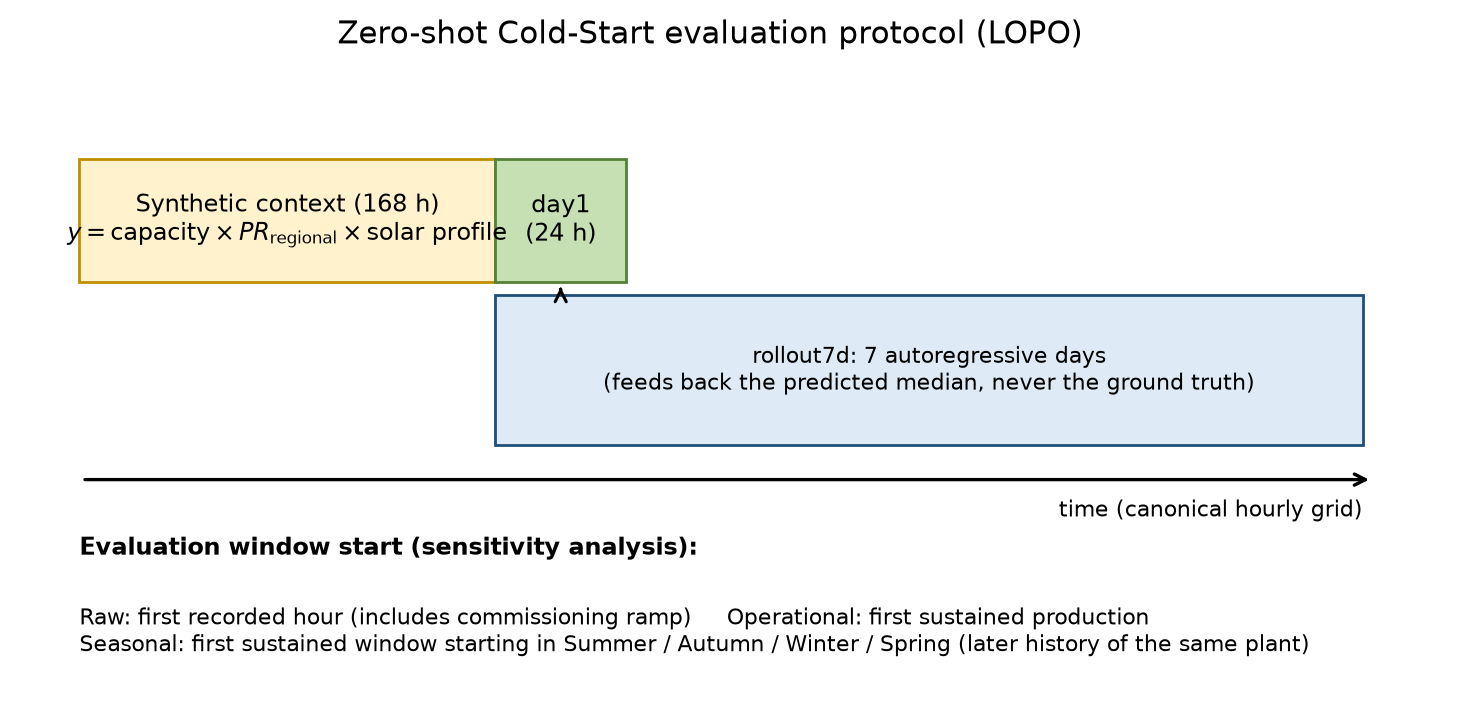
\includegraphics[width=\columnwidth]{fig_method_en.png}
\caption{Zero-shot Cold-Start evaluation protocol. A 168-hour synthetic context seeds the
inference; the model then predicts the \emph{day1} (24\,h) and \emph{rollout7d} horizons.
The window start defines the Raw/Operational/Seasonal sensitivity analysis.}
\label{fig:method}
\end{figure}

\section{Results}
Results correspond to the \emph{total}-scale run: LOPO over the 94 target plants, global
models trained on the complete $N{-}1$ history. Table~\ref{tab:main} reports the operational
window; Fig.~\ref{fig:results} visualizes the weekly roll-out ranking.

\begin{table*}[t]
\centering
\caption{Median performance by configuration --- operational window ($n{=}33$ plants with a
distinguishable commissioning ramp). rRMSE in \%; diurnal coverage of the 90\,\% interval;
pinball P95 in MWh. Best value per column in \textbf{bold}.}
\label{tab:main}
\begin{tabular}{llcccc}
\toprule
Configuration & Scope & rRMSE day1 (\%) & rRMSE roll7d (\%) & Cov$_{90}$ diurnal & Pinball P95 (MWh) \\
\midrule
XGBoost  & Local  & \textbf{40.6} & \textbf{62.2}  & \textbf{0.86} & \textbf{0.033} \\
XGBoost  & Global & 77.5          & 95.4           & 0.99          & 0.091 \\
N-HiTS   & Local  & 73.6          & 104.0          & 0.66          & 0.107 \\
LSTM     & Global & 103.4         & 118.2          & 0.54          & 0.140 \\
Informer & Global & 96.9          & 129.3          & 0.65          & 0.114 \\
TFT      & Global & 110.2         & 133.1          & 0.44          & 0.123 \\
LSTM     & Local  & 102.6         & 146.9          & 0.79          & 0.211 \\
N-HiTS   & Global & 130.6         & 150.4          & 0.36          & 0.277 \\
\bottomrule
\end{tabular}
\end{table*}

\subsection{Point Accuracy}
Three readings emerge from the weekly roll-out. First, \textbf{local XGBoost} is the most
accurate configuration (62.2\,\% median rRMSE), followed by \textbf{global XGBoost}
(95.4\,\%), the best Cross-Site model. Second, among the global deep networks the
\textbf{LSTM} (118.2\,\%) surpasses the attention-based Informer (129.3\,\%) and TFT
(133.1\,\%) and N-HiTS (150.4\,\%)---an ordering consistent with the caution that attention
can be over-provisioned relative to simpler baselines~\cite{Zeng2023}. Third, the
degradation from \emph{day1} to the weekly roll-out is moderate across all families,
indicating that autoregressive median feedback does not destabilize the forecasts.

\begin{figure}[t]
\centering

\includegraphics[width=\columnwidth]{fig_results_en.png}
\caption{Median rRMSE (7-day roll-out, operational window) per configuration. Local models
in green, global Cross-Site models in blue; the dashed line marks the best local baseline.}
\label{fig:results}
\end{figure}

\subsection{Seasonal Sensitivity}
For every plant we build Cold-Start windows starting in each of the four seasons, taken from
its own post-commissioning history (independent of the actual connection season). Winter is
\textbf{systematically the hardest season for every architecture} (Table~\ref{tab:seasonal}):
in the weekly roll-out, global XGBoost rises from 51.8\,\% (summer) to 133.5\,\% (winter) and
local XGBoost from 40.5\,\% to 114.8\,\%. Greater cloud variability and lower mean winter
irradiance weaken the deterministic solar signal and amplify the relative weight of errors,
with a direct operational implication: the forecast uncertainty of a newly connected plant
depends strongly on the season of its commissioning.

\begin{table}[t]
\centering
\caption{Median rRMSE (\%) of the 7-day roll-out by season in which the evaluation window
starts.}
\label{tab:seasonal}
\begin{tabular}{lcccc}
\toprule
Model & Summer & Autumn & Winter & Spring \\
\midrule
XGBoost local  & 40.5 & 35.9 & 114.8 & 101.5 \\
XGBoost global & 51.8 & 53.7 & 133.5 & 106.1 \\
N-HiTS local   & 66.0 & 74.0 & 143.5 & 118.1 \\
LSTM global    & 93.9 & 97.0 & 186.3 & 136.2 \\
TFT global     & 87.7 & 102.0 & 168.8 & 130.9 \\
Informer global & 87.9 & 92.9 & 172.0 & 137.0 \\
N-HiTS global  & 114.0 & 130.3 & 188.7 & 148.9 \\
\bottomrule
\end{tabular}
\end{table}

\subsection{Probabilistic Calibration}
No paradigm calibrates its intervals ideally under the Cold-Start protocol, with deviations
in opposite directions from the 90\,\% nominal (Table~\ref{tab:main}, Cov$_{90}$). Evaluated
on productive hours, the global deep networks are clearly \textbf{under-calibrated} (LSTM
0.54, Informer 0.65, TFT 0.44, N-HiTS 0.36): their bands are too narrow. Global XGBoost, at
the opposite extreme, \textbf{over-covers} (0.99)---bands so wide they rarely fail but lose
operational value, a defect symmetric to the networks', not a virtue. The closest to nominal
is \textbf{local XGBoost} (0.86), whose superiority is confirmed by a much smaller pinball
P95 (0.033 vs.\ 0.091\,MWh for global). The networks' behaviour follows from the design:
each series' local scaler is fit on the synthetic context, whose variance (an idealized
solar profile) is below the real plant variability, producing narrow bands; the local deep
baselines, which see real context, improve (LSTM local 0.79, N-HiTS local 0.66). Post-hoc
recalibration (e.g., conformal prediction) is a clear line of future work.

\subsection{Hypothesis Test}
The hypothesis that the global multi-site model is \emph{more accurate} than a locally
trained model is \textbf{rejected in absolute terms}: no global model reaches the best local
baseline. The single nuance is the matched-architecture comparison. (i) At equal deep
architecture, global transfer is competitive but mixed: global LSTM beats local LSTM
(118.2\,\% vs.\ 146.9\,\%), showing generalized climatic knowledge can exceed limited local
history, yet local N-HiTS beats global N-HiTS (104.0\,\% vs.\ 150.4\,\%). (ii) Against the
mature local baseline, local XGBoost (62.2\,\% roll-out; 40.6\,\% day1) dominates the best
global model (95.4\,\%; 77.5\,\%). (iii) The operational value of the global model lies in
\emph{immediate availability}: the local paradigm needs months of accumulated data, whereas
the global model forecasts usably from the first connected hour---the exact regime that
motivates this work, and one in which no local competitor can exist.

\section{Discussion}
The negative result is itself a contribution: it subjects the widespread belief in global
attentional superiority to a stricter test than usual---target-blind, no local fine-tuning,
against mature local baselines---and demarcates precisely the regime where Cross-Site
transfer retains indisputable value: pure cold start. Several factors plausibly bound the
global models' performance and define the roadmap. \emph{No fine-tuning:} the global model
ran strictly zero-shot while the local baselines that beat it observe real site data; a
two-stage pretrain-then-finetune scheme should close much of the gap as history accrues.
\emph{Intermittency-aware architecture:} the models treat PV as a continuous signal, whereas
it is intrinsically intermittent (deterministic night zeros, stochastic cloud gaps);
explicit intermittency masks in the attention mechanism could redirect representational
capacity to the productive signal. \emph{Corpus scale and compute:} 94 plants and a 6\,GB
training budget may under-serve the higher-capacity TFT/Informer, offering an alternative
explanation for their being outperformed by simpler models. \emph{Interval recalibration}
under transfer (conformal methods) is needed before operational deployment.

\textbf{Limitations.} The study is zero-shot by design (no fine-tuning arm); the rRMSE
normalization inflates absolute magnitudes and is meaningful only in relative comparison;
and operational MLOps deployment is out of scope.

\section{Conclusion}
We benchmarked global Cross-Site transfer against strictly local baselines for cold-start PV
forecasting under a target-blind LOPO protocol over 94 Chilean plants. In absolute accuracy
the global-superiority hypothesis is rejected---a mature local XGBoost remains the model to
beat---but at matched deep architecture global transfer is competitive, and in the pure
cold-start regime it is the only paradigm that produces coherent, immediately available
forecasts. Winter is the hardest season, and the deep networks' probabilistic intervals
require recalibration under transfer. The contribution is not to crown an absolute winner but
to quantify rigorously the trade-off between \emph{immediate availability} and
\emph{asymptotic accuracy} that governs paradigm choice during the commissioning of a new
solar plant.

\section*{Acknowledgment}
This paper condenses the author's undergraduate thesis at Universidad Cat\'olica del Maule,
supervised by Dr.\ Sergio Hern\'andez \'Alvarez. AI-assisted tools supported drafting and
figure preparation; all content, data and results were produced and verified by the author.

\bibliographystyle{IEEEtran}
\bibliography{paper}

\end{document}
